In this section we are going to describe the system that we are going to work on (the system for which we want to compute RT surfaces) which features interface CFTs. We start by summarizing results of \cite{Bachas_2021}, where two CFTs were considered separated by an interface. The dual geometry features a domain wall separating two classical geometries which could be part of thermal AdS or BTZ black hole geometry. Since the general system can be in numerous phases, we prefer to consider only one phase. We take the limit of some large canonical variables and Lagrangian parameters to determine the dominant phase in that case. We use the same notations as \cite{Bachas_2021}.

\section{The general system}\label{general system}

We consider two conformal field theories, CFT$_1$ and CFT$_2$, on a circle at thermal equilibrium $T$. The two CFTs are characterized by their central charges, $c_1$ and $c_2$ respectively, and are separated by an interface characterised by its tension $\lambda$. In addition to that, there are two additional parameters, and these are the sizes of the regions occupied by the two CFTs: $L_1$ and $L_2$. We refer to the side with size $L_1$ as the red slice and the one with size $L_2$ as the blue slice as in fig. \ref{ICFT}.

\begin{figure}[h!]
    \centering
    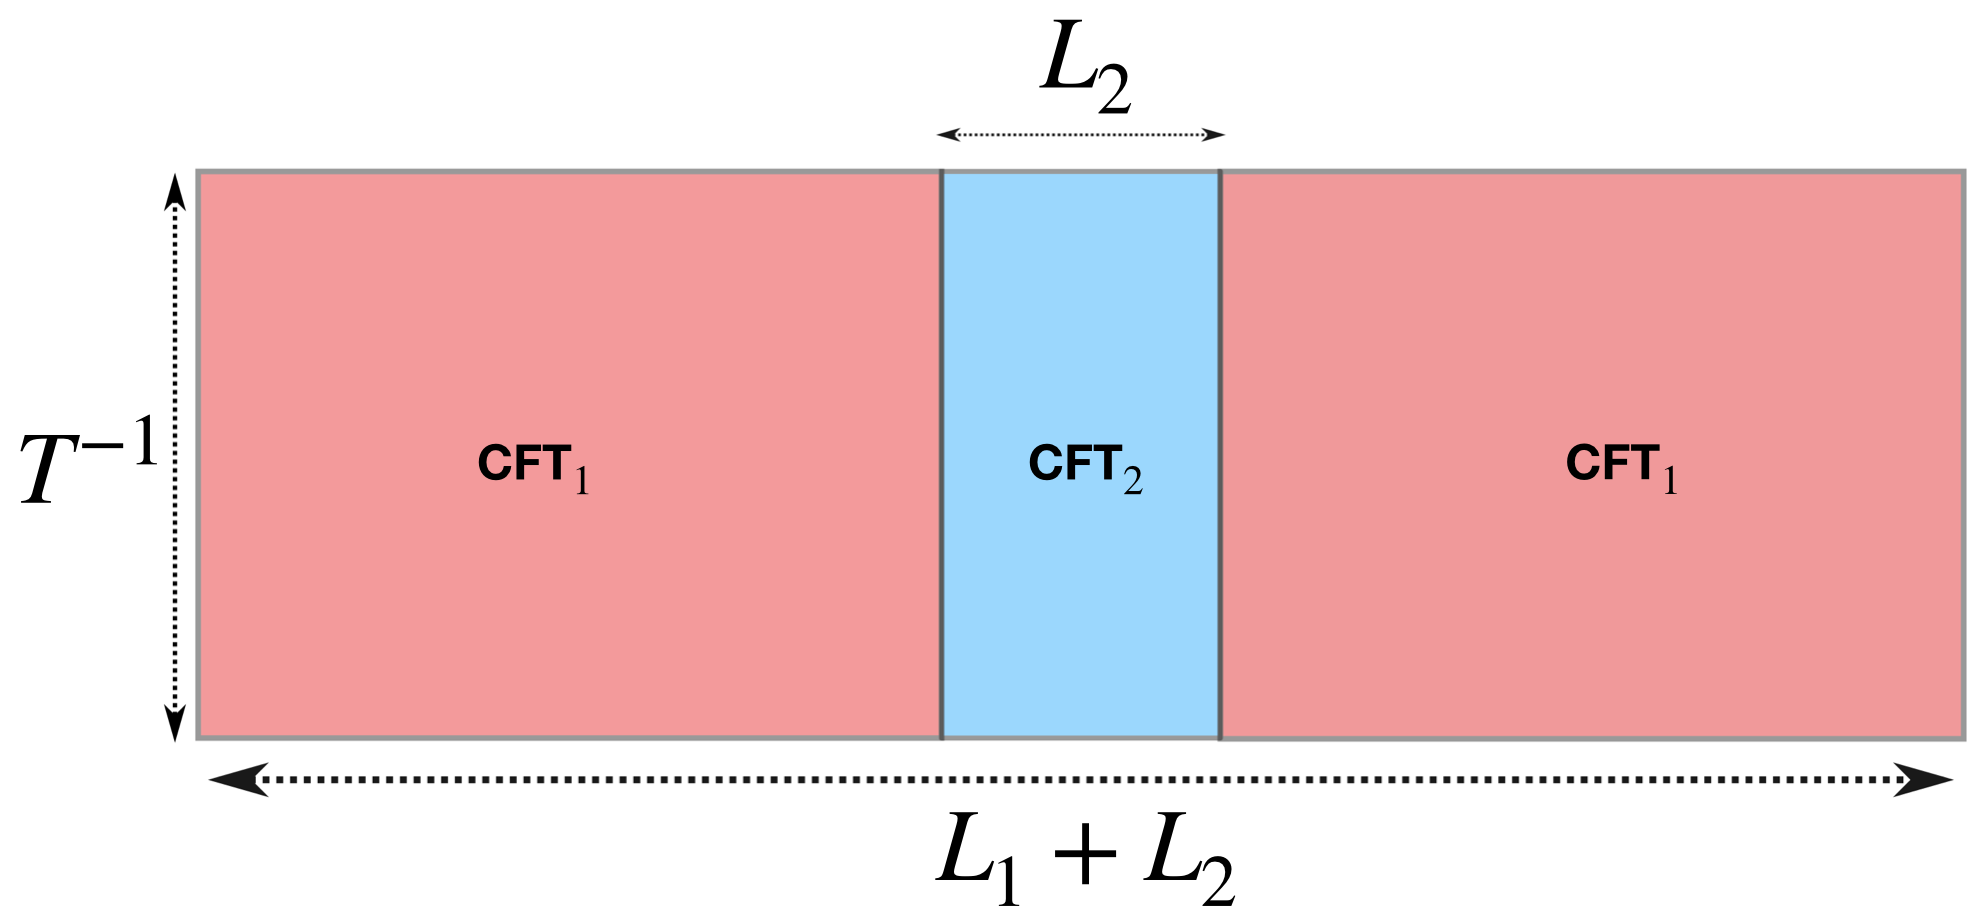
\includegraphics[width=0.65\textwidth]{figures/ICFTb.png}
    \caption{AdS boundary with 2 CFTs separated by an interface. Space and Euclidean time are compact. The red region was intentionally made larger than the blue one as we will tend to consider the case $L_1\gg L_2$ lately.}
    \label{ICFT}
\end{figure}

The two regions extend in the interior to gravitational solutions with different topologies, separated by a domain wall. The action is that given in (\ref{action cft}). The AdS radii $\ell_i$ are related to the central charges via $c_i = 12\pi\ell_i$. We work in Planck units where $8\pi G = 1$.

The boundary is extended in the interior into gravitational solutions of two types: thermal AdS or BTZ black hole. The two slices can be parts of these solutions, having several topologies as presented in fig. \ref{topologies}. The solution could be part of thermal AdS$_3$, either with a center $($E$1)$ or centerless $($E$2)$, or could be part of a BTZ black hole, either with a complete horizon $($H$1)$ or a part of it $($H$2)$ or horizonless $($E$2')$.

\begin{figure}
    \centering
    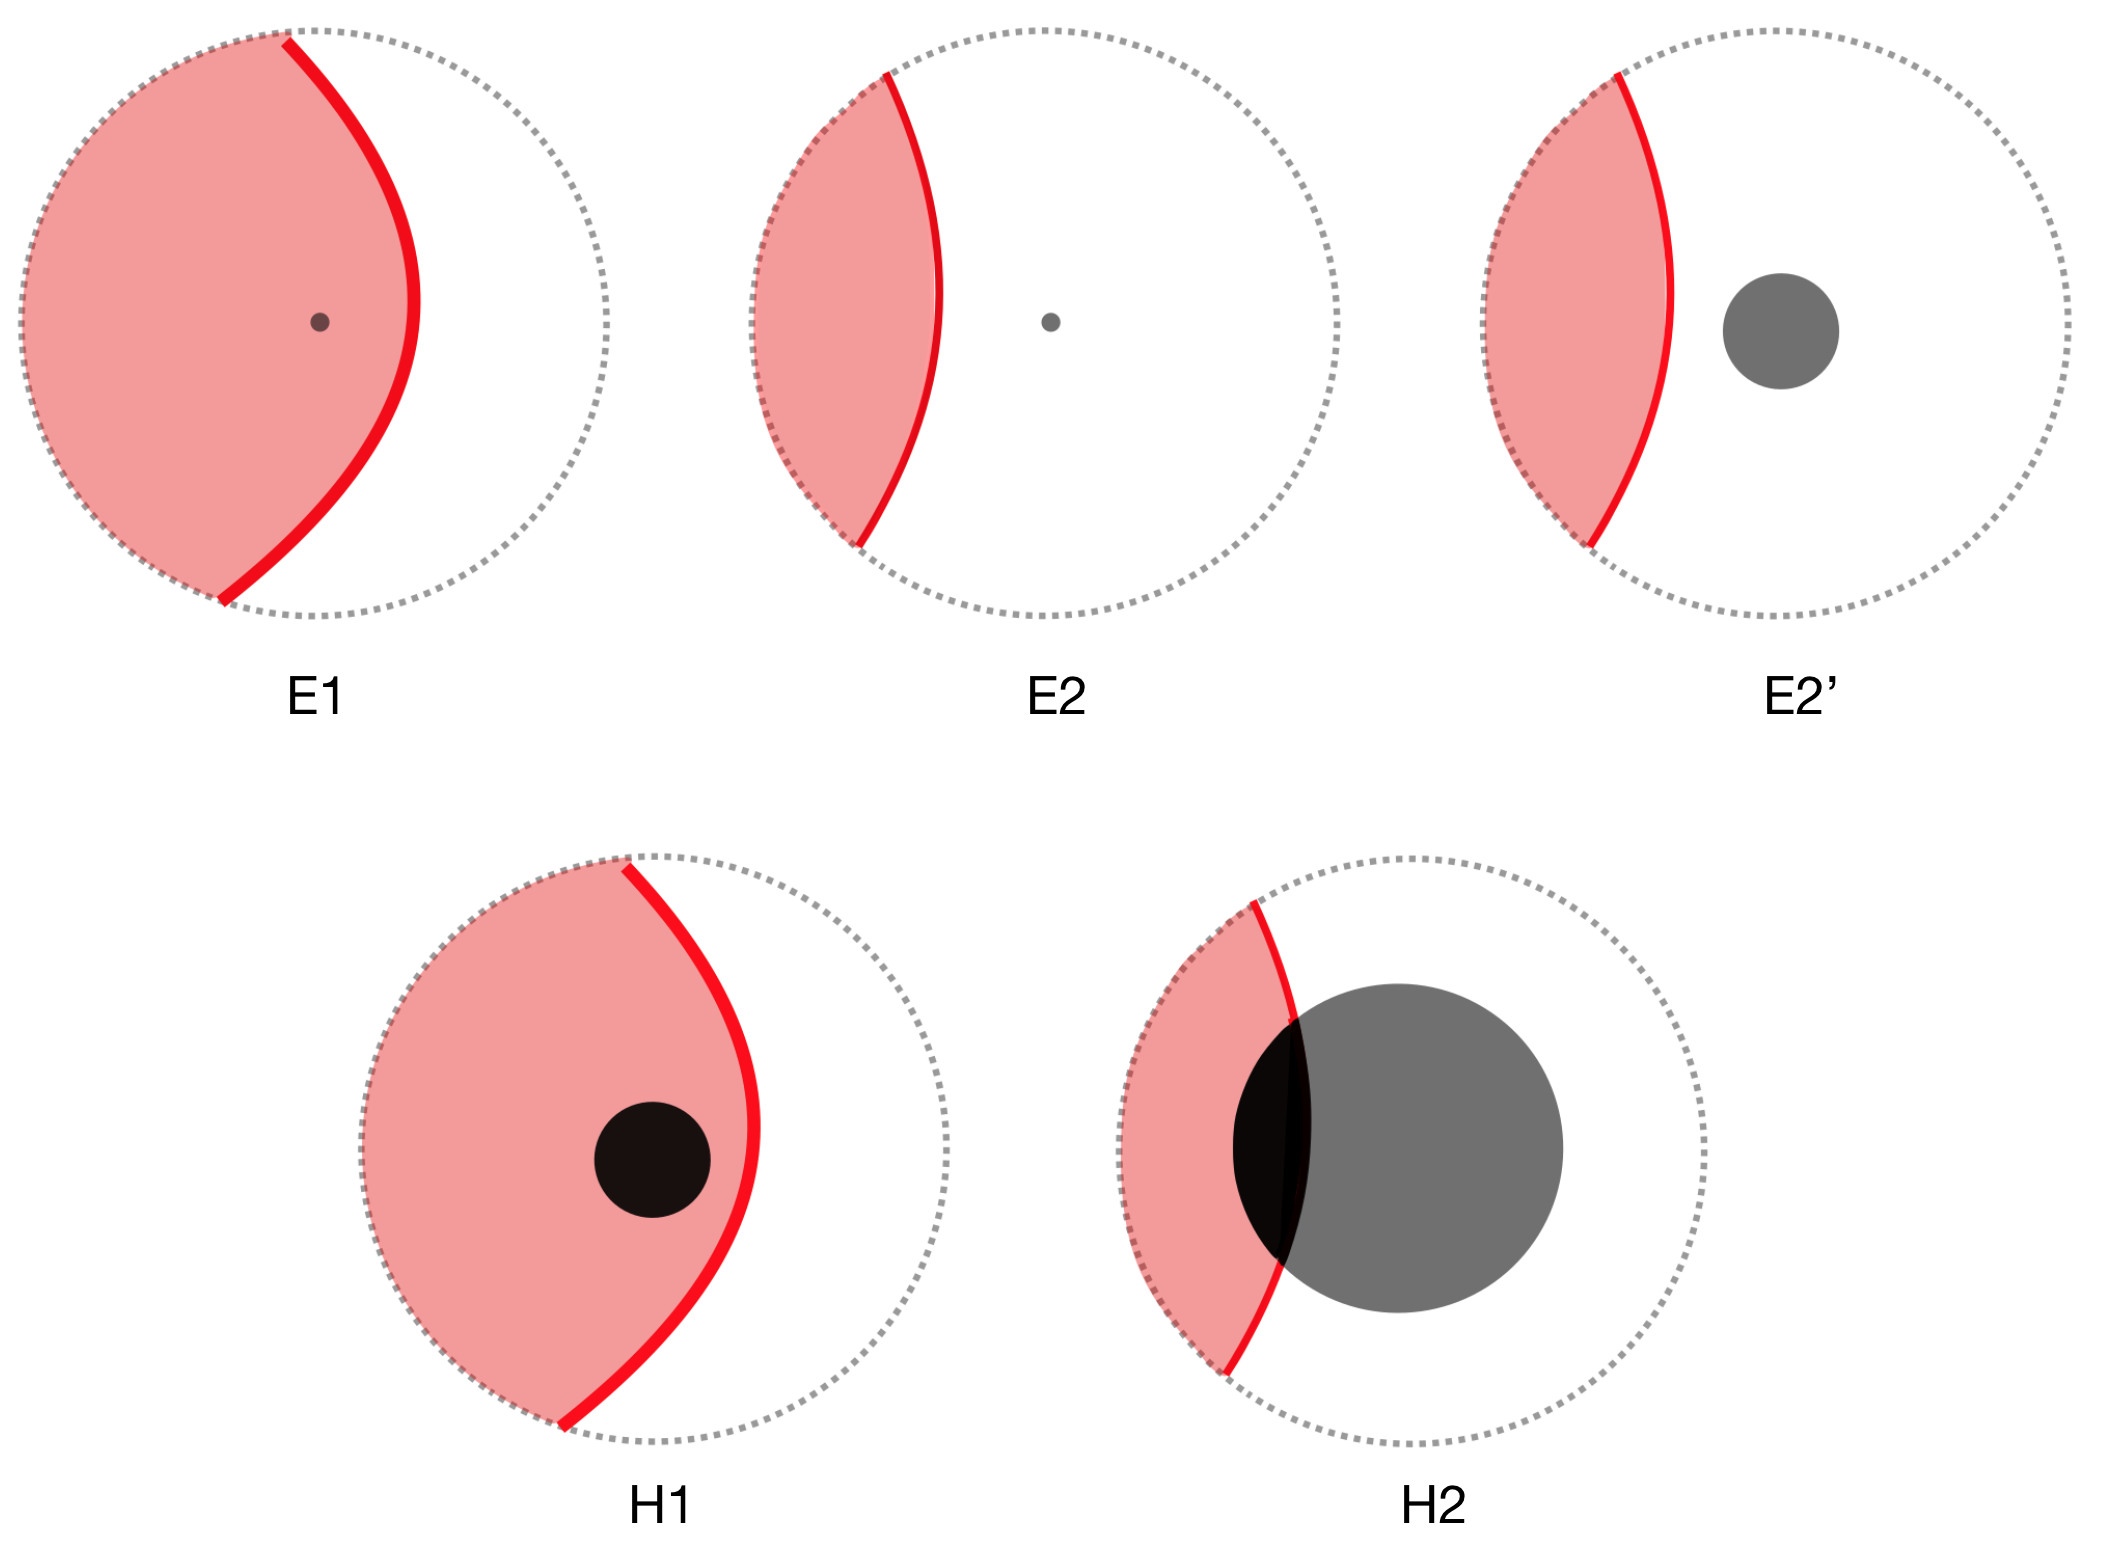
\includegraphics[width=0.65\textwidth]{figures/phasesred.png}
    \caption{Different topologies depending on the geometry (thermal AdS or BTZ) and the wall. We represent the solutions for the red slice, while the blue slice is supposed to have the same solutions.}
    \label{topologies}
\end{figure}

We write the metric in terms of two coordinate charts $\left(x_j,r_j\right)$ and the globally defined time $t$:
\begin{equation}\label{geometry}
    \text{d}s^2 = \frac{\ell_j^2}{r_j^2-M_j\ell_j^2}\text{d}r_j^2 - \left(r_j^2-M_j\ell_j^2\right)\text{d}t^2+r_j^2\text{d}x_j^2
\end{equation}
with $\left(x_j,r_j\right)\in \Omega_j$, where $\Omega_j$ is the range of coordinates in each slice, determined by the wall, the horizon (when it exists) and the cutoff surface $r_j\sim 1/\epsilon$.

There are two important points to notice. The first one is that regularity requires that for H$1$ and H$2$ slices we have $M_j=\left(2\pi T\right)^2$. The second point is that there is no topological difference between E$2$ and E$2'$. These two solutions differ only by the sign of the mass $M_j$.

A change of coordinates that will be used later is,
\begin{align}\label{change of coord rz}
    r_j=\frac{1}{z_j},         &&           t=T_j\ell_j,          &&        x_j=\phi_j\ell_j.
\end{align}

In these new coordinates the metric (\ref{geometry}) takes the form
\begin{equation}\label{geometry z}
    \text{d}s^2 = \frac{\ell_j^2}{z_j^2}\left(\frac{1}{f_j(z_j)}\text{d}r_j^2 - f_j(z_j)\text{d}T_j^2+\text{d}\phi_j^2\right),
\end{equation}
where $f_j(z_j)=1-\frac{z^2}{{z_j}_h^2}$ and ${z_j}_h=\frac{1}{\ell_j\sqrt{M_j}}$.

\section{The wall equation}

\subsection{Determining the range of $\lambda$}

The different parameters of our system, the mass parameters $M_j$, the AdS radii $\ell_j$, and the tension of the wall $\lambda$, must obey different equations. A set of these equations are the matching conditions. They guarantee that there is a well defined metric on the wall. These are given by matching the metric of the two slices at the wall as was presented in \cite{Simidzija_2020,Bachas_2021}:
\begin{align}
    &r_j^2-M_j\ell_j^2=f(\sigma) \label{matching condition 1} \\
    f&^{-1}\ell_1^2r'_j^2 + r_j^2x'_j^2 = g(\sigma) \label{matching condition 2}
\end{align}
where the prime corresponds to a derivative with respect to $\sigma$ the wall parameter. The two functions $f(\sigma)$ and $g(\sigma)$ are the diagonal terms of the wall induced metric, $\text{d}\hat{s}^2=-f(\sigma)\text{d}t^2+g(\sigma)\text{d}\sigma^2$. The other matching condition, known as the Israel-Lanczos\cite{Israel:1966rt} matching condition, can be written as:
\begin{equation}\label{Israel-lanczos}
    \frac{r_1^2x'_1}{\ell_1} +  \frac{r_2^2x'_2}{\ell_2} = \lambda\sqrt{fg}.
\end{equation}

Solving (\ref{matching condition 1}), (\ref{matching condition 2}) and (\ref{Israel-lanczos}) near the boundary, where $M_j$ can be neglected, is not complicated. The solution gives the possible values of $\lambda$ for a static solution. We find that $\lambda$ has a minimum and a maximum value:
\begin{equation}\label{domain wall}
    \lambda_{\text{min}} <\lambda< \lambda_{\text{max}},
\end{equation}
where the critical tensions  are,
\begin{align}
     \lambda_{\text{min}} = \frac{1}{\ell_1} - \frac{1}{\ell_2} &&  \lambda_{\text{max}} = \frac{1}{\ell_1} + \frac{1}{\ell_2}.
\end{align}
The complete derivation can be found in \cite{Bachas_2021}, section 4.

\subsection{General solutions}\label{solutions}

The general solutions of (\ref{matching condition 1}), (\ref{matching condition 2}) and (\ref{Israel-lanczos}) are found by considering a convenient parametrization of the wall outside the horizon, see \cite{Bachas_2021}. The solutions are the following:
\begin{subequations}
\label{wall solution}
\begin{align}
     r_j &= \sqrt{|\sigma| + M_j\ell_j^2},\label{solution r} \\
     \frac{x'_1}{\ell_1} &= -\frac{\sigma\left(\lambda^2+{\lambda_0}^2\right)+M_1-M_2}{2\left(\sigma+M_1{\ell_1}^2\right)\sqrt{A\sigma\left(\sigma-\sigma_+\right)\left(\sigma-\sigma_-\right)}},\label{solution x1} \\
     \frac{x'_2}{\ell_2} &= -\frac{\sigma\left(\lambda^2-{\lambda_0}^2\right)+M_2-M_1}{2\left(\sigma+M_2{\ell_2}^2\right)\sqrt{A\sigma\left(\sigma-\sigma_+\right)\left(\sigma-\sigma_-\right)}}, \label{solution x2}
\end{align}
\end{subequations}
where $A = \left({\lambda_\text{max}}^2-{\lambda}^2\right)\left(\lambda^2-{\lambda_\text{min}}^2\right)$ and $\sigma_\pm$ are poles of $g(\sigma)$.

The above equations give solutions of the wall equation in terms of the mass parameters $M_j$. These parameters are not free to choose. They must obey the Dirichelet boundary conditions:
\begin{gather}\label{Dirichelet bc}
    L_j = 2{\int_{\sigma_+}}^\infty \text{d}\sigma\,x'_j \quad \text{for     E2, E2}'; \\
    L_j = nP_j + 2{\int_{\sigma_+}}^\infty \text{d}\sigma\,x'_j \quad \text{for     E1, H1;} \\
    L_j = \Delta x_j|_\text{Hor} + 2{\int_{\sigma_+}}^\infty \text{d}\sigma\, x'_j \quad \text{for     H2.}\label{Dirichelet hot}
\end{gather}
where $P_j$ is the period of $x_j$, $n$ the winding number and $\Delta x_j|_\text{Hor}$ is Horizon arc in the $j$th slice

\section{Allowed phases}\label{tablesec}

From the different topologies described in section \ref{general system}, only some of theme can be paired together. These are results of three no-go lemmas\footnote{See section 5 of \cite{Bachas_2021}.}. The possible phases are described in fig. \ref{table}.

\begin{figure}
    \centering
    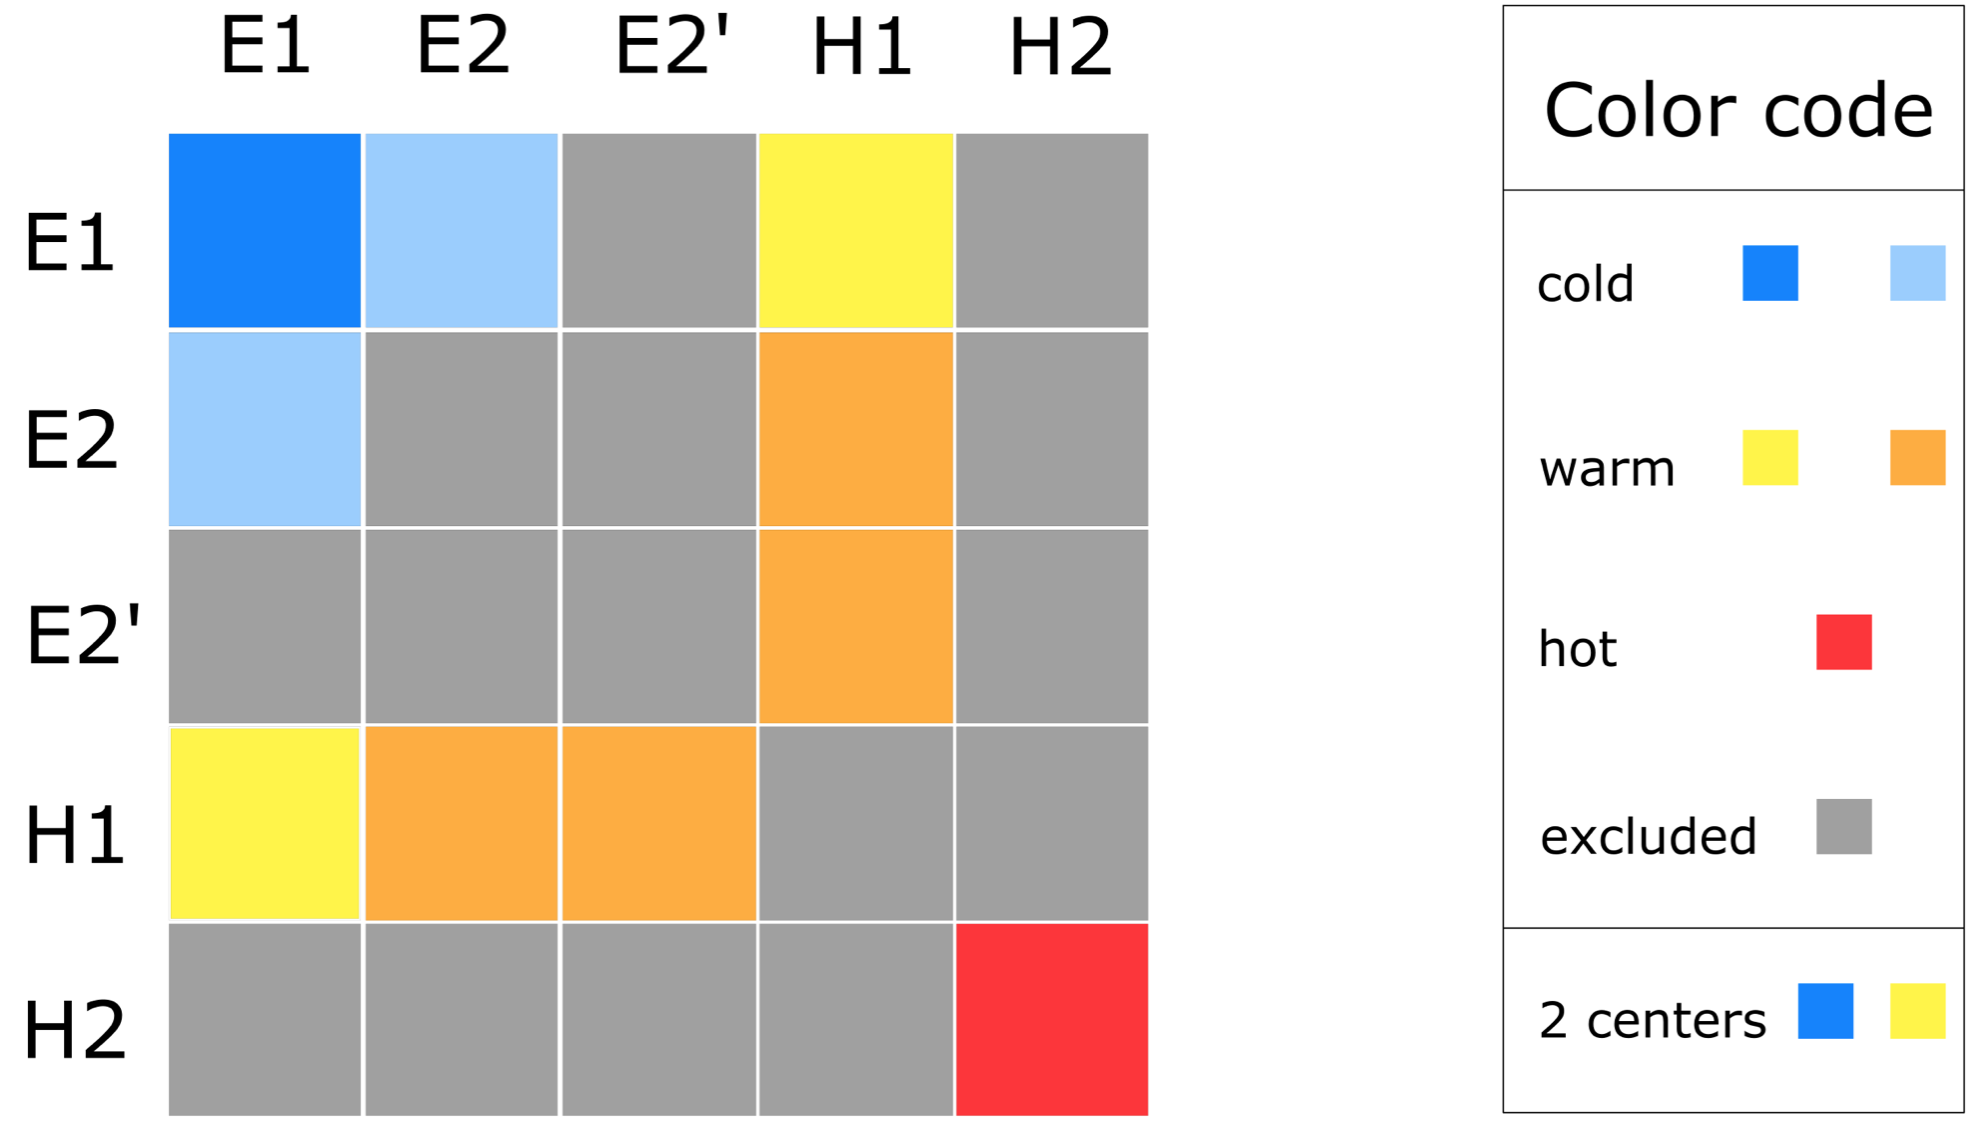
\includegraphics[width=0.65\textwidth]{figures/table.png}
    \caption{Phases of the domain-wall spacetime. The type of the red slice labels the rows of the table, and that of the blue slice the columns.}
    \label{table}
\end{figure}

We use the notation $[$X$_1$,X$_2]$ to describe a solution with X$_1$ topology in the red side and X$_2$ topology in the blue slice. Note that two of the allowed phases are double centered, one is cold $\left[\text{E}1,\text{E}1\right]$ and the other one is the warm one $\left[\text{E}1,\text{H}1\right]$. 

Another point to mention is that horizons are more likely to form in the true vacuum, i.e the slice with the smallest ground state energy. This energy can be computed by means of the stress energy tensor and is found to be an increasing function of the central charge,
\begin{equation}
    E_0 \propto -\frac{1}{c^2}.
\end{equation}
In \cite{Bachas_2021}, it was shown numerically that solutions with horizons on the false vacuum side cease to exist as we surpass the the critical value $b=\frac{\ell_2}{\ell_1}=3$.

\section{The limit of Large $L_1$ and $\ell_2$}\label{limit}

We want to create a system where a part of it is characterised with a large number of degrees of freedom, coupled to a very large region modeling a bath. We take the limit of large central charge for the blue slice $\ell_1\ll \ell_2$, and large boundary region for the red slice $L_1\gg L_2$. We also consider $\lambda\rightarrow\lambda_{\text{min}}$ so the wall can be as transparent as possible. We want to find which of the phases described in the previous section is the dominant one in this limit.

In order to determine the dominant phase, we think thermodynamics, where we have fixed Lagrangian parameters $\lambda$ and $\ell_j$, and canonical variables that determine the state, $T$ and $L_j$. Because of scale invariance, we work with four dimensionless parameters,
\begin{align}
    \tau_j:=TL_j, && \gamma:= \frac{L_1}{L_2}, && \text{and} \quad \mu := \frac{M_2}{M_1}.
\end{align}

The energy and Entropy of each subsystem is given by
\begin{equation}
    E_j = \frac{L_j\ell_j}{2}M_j \quad \text{and} \quad S_j = 2\pi\ell_j\sqrt{M_j}\Delta x_j|\text{Hor}.
\end{equation}

The dominant phase is the one that has the lowest free energy,
\begin{equation}
    F = \sum_j E_j -T S_j.
\end{equation}

The free energy can be computed in terms of $\tau$, using the boundary conditions (\ref{Dirichelet bc}).

\subsection{Possible solutions}

In the limit we are working on, we have $\gamma,\tau \gg 1$. In this case we can already rule out cold solutions of type $\left[\text{E}1,\text{E}1\right]$, $\left[\text{E}1,\text{E}2\right]$ and $\left[\text{E}2,\text{E}1\right]$.
 
We are left with the warm and hot solutions. These are $\left[\text{H}1,\text{E}1\right]$, $\left[\text{H}1,\text{E}2\right]$, $\left[\text{H}1,\text{E}2'\right]$ and $\left[\text{H}2,\text{H}2\right]$. As we have mentioned in the end of section \ref{tablesec}, we have ruled out the solutions with H1 on the blue side since the red side is the true vacuum, $\ell_1\ll\ell_2$.
 
We can also rule out $\left[\text{H}1,\text{E}1\right]$. The difference between E$1$ (with a center) and E$2$ (centerless) is the sign of $x_2'$ at the turning point $\sigma_+$, which is
\begin{equation}
    \text{sign}(x_2')|_{\sigma_+} = 
    \left\{
    \begin{array}{lll}
        -1 & \mbox{if} & X_2=\text{E}1, \\
        +1 & \mbox{if} & X_2=\text{E}2.
    \end{array}
\right.
\end{equation}

If we consider the case of light walls $\lambda\rightarrow\lambda_{\text{min}}$ and since $X_1=$H$1$, we can see from (\ref{solution x2}) that $x_2'(\sigma)>0$ at $\sigma_+$. We are therefore in the case $X_2=$E$2$. The condition $\lambda<\lambda_0$ is sufficient.

\subsection{The free energy}

In order to determinant the dominant phase of the rest of the allowed phases, we have to compare their free energies. The general form of the free energy was already introduced in section \ref{limit}. The three free energies that we are interested in have the same divergent term (the term proportional to $L_1$). This part can be omitted.

The expression of the free energies are then:
\begin{subequations}\label{free E}
    \begin{align}
        \Tilde{F}\left(\left[\text{H}1,\text{E}2\right]\right) &=\frac{\ell_2}{L_2}\left( \frac{1}{2}\mu\left(\tau_2\right)\left(2\pi\tau_2\right)^2 - \frac{2\pi}{{b}}\Tilde{f}_1(\tau_2)\tau_2\right), \label{F(E2)}\\
        \Tilde{F}\left(\left[\text{H}1,\text{E}2'\right]\right) &=\frac{\ell_2}{L_2}\left( \frac{1}{2}\mu\left(\tau_2\right)\left(2\pi\tau_2\right)^2 - \frac{2\pi}{{b}}\Tilde{f}_1(\tau_2)\tau_2\right), \label{F(E2')}\\
        \Tilde{F}\left(\left[\text{H}2,\text{H}2\right]\right) &=\frac{\ell_2}{L_2}\left( -\frac{1}{2}\left(2\pi\tau_2\right)^2 - (2\pi)^2\left(\frac{g_1\left(\lambda\right)}{b}+g_2\left(\lambda\right)\right)\tau_2\right). \label{F(H2)}
    \end{align}
\end{subequations}
$b$ is the ratio of the two central charges $b=\ell_2/\ell_1$. The difference between $\Tilde{F}\left(\left[\text{H}1,\text{E}2\right]\right)$ and $\Tilde{F}\left(\left[\text{H}1,\text{E}2\right]\right)$ lies in the sign of $\mu$ which is negative for (\ref{F(E2)}) and positive, yet smaller than 1, for (\ref{F(E2')}). By $\Tilde{F}$ we mean "$F-\text{divergent part}$", which is 
\begin{equation}
    \Tilde{F} = F + \frac{\ell_1L_1}{2}(2\pi T)^2.
\end{equation}

Note that $\mu$, the ratio of the two masses, depends on $\tau_2$ through $f_2$, while it is equal to 1 in the hot phase. The functions $\Tilde{f}_i$ are rewritten versions of the boundary conditions (\ref{Dirichelet bc}). The full derivation of their expression is detailed in appendix \ref{appendix D}.
\begin{align}\label{f2 constrain}
     2\pi T\Delta\big|_\text{Hor} -2\pi\tau_1= \Tilde{f}_1(\mu), && 2\pi\tau_2= -\Tilde{f}_2(\mu).
\end{align}

The function $\Tilde{f}_2(\mu)$ can be expressed in terms of the Elliptic integrals of the first, second and third kind,
\begin{equation}
    \Tilde{f}_2(\mu) = \frac{2\ell_2}{\sqrt{As_+}}\left[\frac{1-\mu}{s_+ u}\left(\bm{K}(\nu)-\bm{\Pi}(u,\nu)\right)+\left(\lambda^2-\lambda_0^2\right)\bm{\Pi}(u,\nu)\right],
\end{equation}
where $s_\pm=\sigma_\pm/M_1$, $\nu=s_-/s_+s$ and $u=-\mu\ell_2^2/s_+$. The limit of $\Tilde{f_2}$ when $\mu\rightarrow0$ is well defined,
\begin{equation}
    \Tilde{f}_2(\mu=0) = \frac{2\ell_2}{\sqrt{As_+}}\left[\frac{1}{s_-}\left(\bm{E}(\nu)-\bm{K}(\nu)\right)+\left(\lambda^2-\lambda_0^2\right)\bm{K}(\nu)\right].
\end{equation}

The variable $\nu$ takes values in $(-\infty,0)$ and therefore the Elliptic integrals of the first and second kind are well behaved. The $\bm{\Pi}(u,\nu)$ integral diverges for $u=1$. This is the case when the string turning point and the the AdS center coincide $\sigma_+ = -M_2\ell_2^2$. This point specifies a sweeping transition between a center-less topology E2 and a center-full topology E1. This equation has one solution,
\begin{equation}\label{sweeping trans}
    \mu^* = \frac{1/b^2}{1-\ell_1^2\lambda}.
\end{equation}
Since both topologies E1 and E2 belong to part of thermal AdS geometry while the red side is fixed at H1, this sweeping transition between E1 and E2 happens at negative value of $\mu$. A sufficient condition to avoid this solution (\ref{sweeping trans}) is to take $\lambda\in(\lambda_\text{min},1/\ell_1))$. In this case $\mu^*>0$ and therefore the value $u=1$ is avoided.

Note that the function $\Tilde{f}_2(\mu)$ converges to 0 when $\mu\rightarrow-\infty$. This can be seen just by computing the limit of $s_+(\mu)\rightarrow\infty$. In conclusion, $\Tilde{f}_2$ is a negative finite function of $\mu$. As seen from equation (\ref{f2 constrain}), this function constrains the values of $\tau_2$ in the case of warm phases with centerless blue slices. As it takes only values in $(0,-\min\{\Tilde{f}_2\})$, the warm solutions will cease to exist for high $\tau_2$, i.e high $T$.

The hot phase $\left[\text{H}2,\text{H}2\right]$ is constrained by the existence of the horizon on both sides, i.e $\Delta x_j|_{Hor}\geq0$. Solving this inequality, we get a lower bound for $\tau_2$,
\begin{equation}
    \tau_2\geq\frac{1}{\pi}\tanh^{-1}\left(\frac{\ell_2(\lambda_0^2-\lambda^2)}{2\lambda_0}\right):=\tau_2^*.
\end{equation}
The hot solution will exist for any temperature higher than $\tau_2^*$ and therefore will be the only existing solution for $\tau_2\geq\max\left\{\tau_2^*,-\min\{\Tilde{f}_2\}\right\}$. This could be seen as analogous to a Hawking-Page transition where we take the temperature to be higher than some critical value in order to have a dominant solution in which a horizon exists in the blue slice.

\subsection{Example}

\begin{figure}
    \centering
    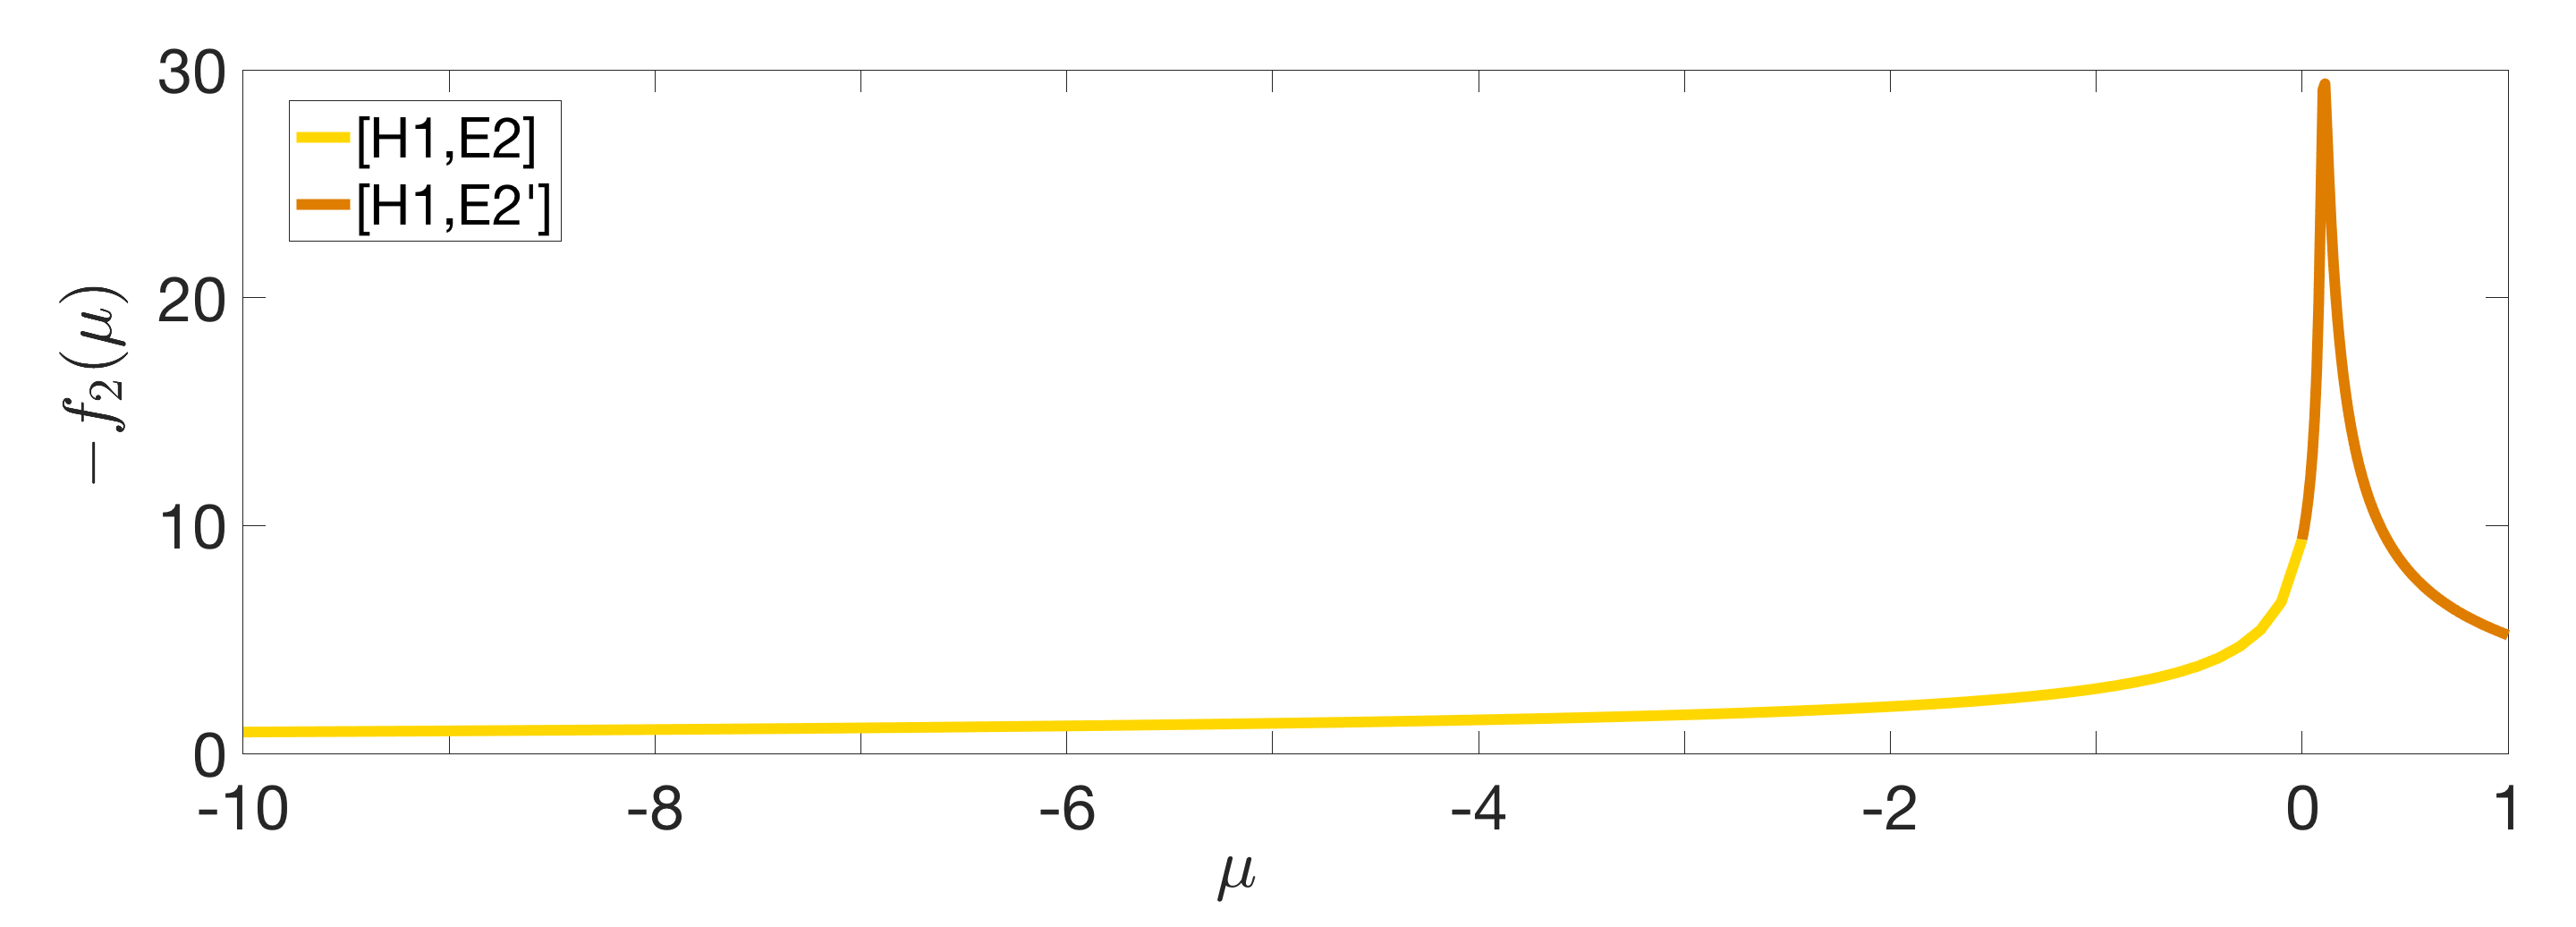
\includegraphics[width=0.9\textwidth]{figures/f2.png}
    \caption{The function $-\Tilde{f}_2(\mu)$ which determines $\tau_2$ through eq. (\ref{f2 constrain}). The point $\mu = 0$ represents the limit between the two warm phases. The function $\Tilde{f}_2(\mu)$ goes to zero for $\mu\rightarrow-\infty$.}
    \label{f2}
\end{figure}

Let's consider a special case and choose some values of $\ell_1$ and $\ell_2$. We choose,
\begin{align}
    \ell_1 = 1, && \ell_2 = 10 && \text{and} && \lambda = \lambda_{\text{min}} + \frac{1}{100\ell_2}.
\end{align}

We plot $\Tilde{f}_2$ as a function of $\mu$ in fig. \ref{f2} with $\mu$ ranging from $-\infty$ to $1$. We see that the function $\Tilde{f}_2$ is negative as discussed before and has a minimum value at $\mu = \Tilde{\mu}>0$. From the shape that $\Tilde{f}_2(\mu)$ takes, we can determine some ranges of $\tau_2$ where warm phases can exist.

The function $\Tilde{f}_2$ for positive $\mu$ takes values between $\min\left\{\Tilde{f}_2(\mu)\right\}=\Tilde{f}_2(\Tilde{\mu})$ and $\max\left\{\Tilde{f}_2(\mu)\right\} = \Tilde{f}_2(1)$. This constrains the values of $\tau_2$ under which the phase $\left[\text{H}1,\text{E}2^{\prime}\right]$ can exist,
\begin{equation}
    -\Tilde{f}_2(1)\leq 2\pi\tau_2\leq - \Tilde{f}_2(\Tilde{\mu}).
\end{equation}

On the $\mu\leq 0$ side of the plot \ref{f2}, the function $-\Tilde{f}_2(\mu)$ is only increasing, having its minimum 0 when $\mu\rightarrow-\infty$ and its maximum at $-\Tilde{f}_2(0)$. Therefore, the warm phase $\left[\text{H}1,\text{E}2\right]$ exists for
\begin{equation}
    0 \leq 2\pi\tau_2\leq - \Tilde{f}_2(0).
\end{equation}

So in summary, we have a region where only $\left[\text{H}1,\text{E}2^\prime\right]$ exists, another region where only $\left[\text{H}1,\text{E}2\right]$ exists, and in between them a region where the two phases coexist. The hot phase on the other hand only exists for $\tau_2\geq\tau_2^*$. Note that when we say only a warm phase exists, we don't exclude the existence of the hot phase nor the cold phases. The results are summarized in table \ref{summary}.
\begin{table}
    \centering
    \begin{tabular}{ |c|c|c|c| } 
        \hline
        $2\pi\tau_2$ & 0 $\rightarrow -\Tilde{f}_2(1)$ & $-\Tilde{f}_2(1) \rightarrow -\Tilde{f}_2(0)$ &  $-\Tilde{f}_2(0) \rightarrow \Tilde{f}_2(\Tilde{\mu})$\\ 
        & & & \\
        \text{Phases} & $\left[\text{H}1,\text{E}2\right]$ & $\text{both}$ & $\left[\text{H}1,\text{E}2^\prime\right]$ \\ 
        \hline
    \end{tabular}
    \caption{The values of $\tau_2$ are separated in three intervals, where each one is characterized with a different phase.}
    \label{summary}
\end{table}

\begin{figure}
    \centering
    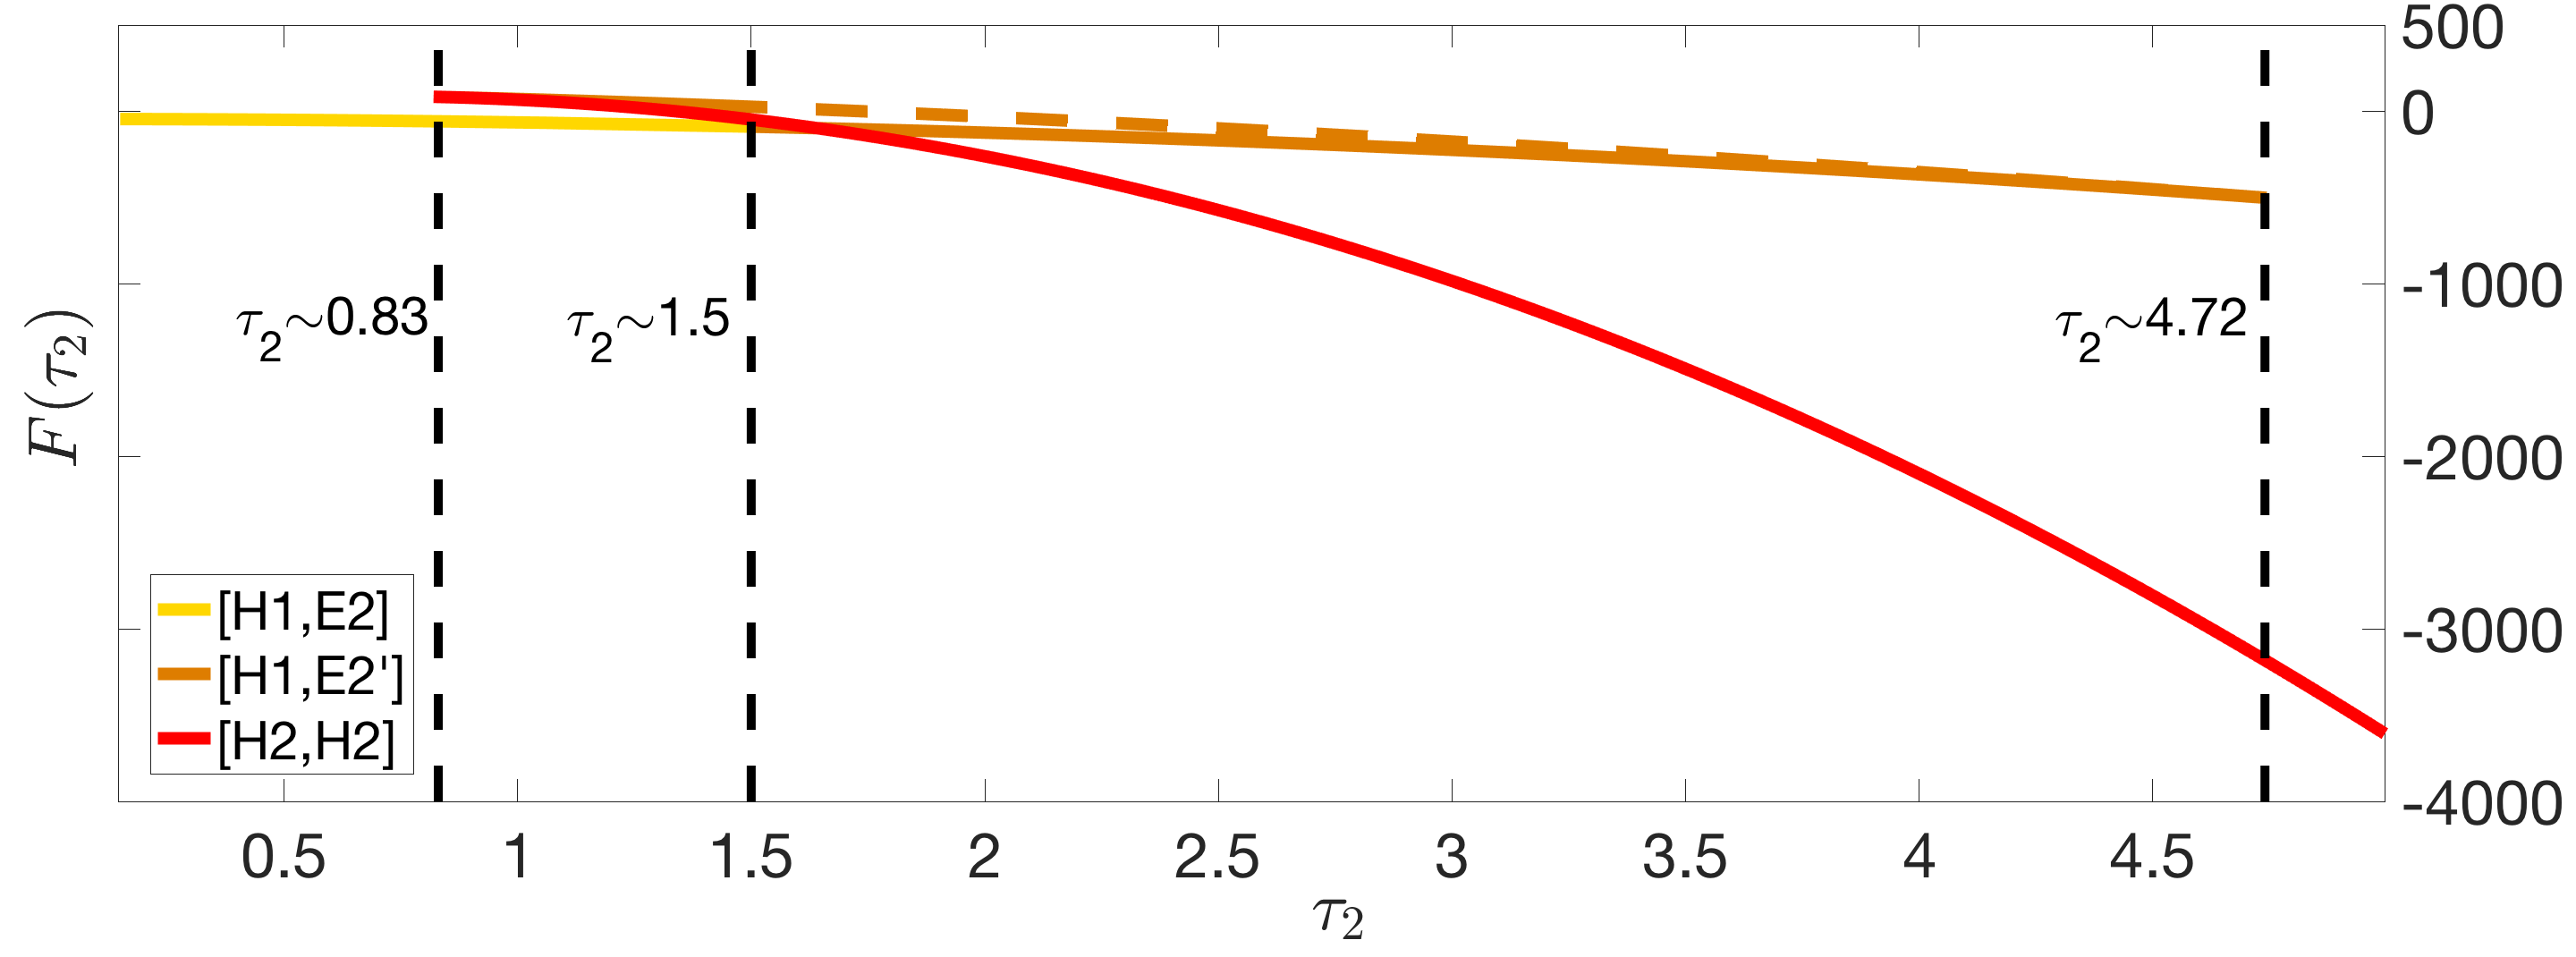
\includegraphics[width=0.9\textwidth]{figures/Free_energy_2.png}
    \caption{The free energies (\ref{free E}) of the three phases (warm and hot) as a function of $\tau_2$. The value of the free energy of $\left[\text{H}2,\text{H}2\right]$ keeps on reaching higher negative values as $\tau_2$ increases. The free energy \ref{F(E2')} takes two values for $\tau_2>1.5$ due to the shape of $f_2(\mu)$. We only consider the minimum of the two values.}
    \label{free_energie}
\end{figure}

We plotted the three free energies in figure \ref{free_energie}. We can see that as we start with low temperature, i.e lower $\tau_2$, the only phase that exist is $\left[\text{H}1,\text{E}2\right]$ while $\left[\text{H}1,\text{E}2'\right]$ and the hot phase do not appear yet. As $\tau_2$ increases, the hot phase and $\left[\text{H}1,\text{E}2'\right]$ appear, but they are dominated by $\left[\text{H}1,\text{E}2\right]$. At $2\pi\tau_2=-\Tilde{f}_2(1)$, $\left[\text{H}1,\text{E}2\right]$ ceases to exist and a continuous phase transition happens between the two warm phases. Shortly after that, the hot phase $\left[\text{H}2,\text{H}2\right]$ takes over and remains dominant for higher $\tau_2$.

\section{The Geometry of the hot phase}
The hot phase seems to dominate over the warm phases early and continues to exist for higher temperature while the warm phases cease to exist. Therefore we consider $\left[\text{H}2,\text{H}2\right]$ to be the dominant phase that we intend to study in the next chapters. We start by writing explicitly its geometry.

The geometry was already written in eq. (\ref{geometry}). In order to determine the range of the coordinates $\left(x_j,r_j\right)\in \Omega_j$, we have to solve the wall equation in section \ref{solutions}. The wall parameter $\sigma$ takes values in $(-\infty,-\sigma_+)\cup(\sigma_+, \infty)$. In the case of the hot phase $\sigma_+=0$. From eq. (\ref{solution r}), we can see that $r_j$ takes values in $(\ell_j\sqrt{M_j},\infty)$, which are exactly the values outside the horizon. Regularity of the geometry requires $M_1=M_2=(2\pi T)^2$.

\begin{figure}
    \centering
    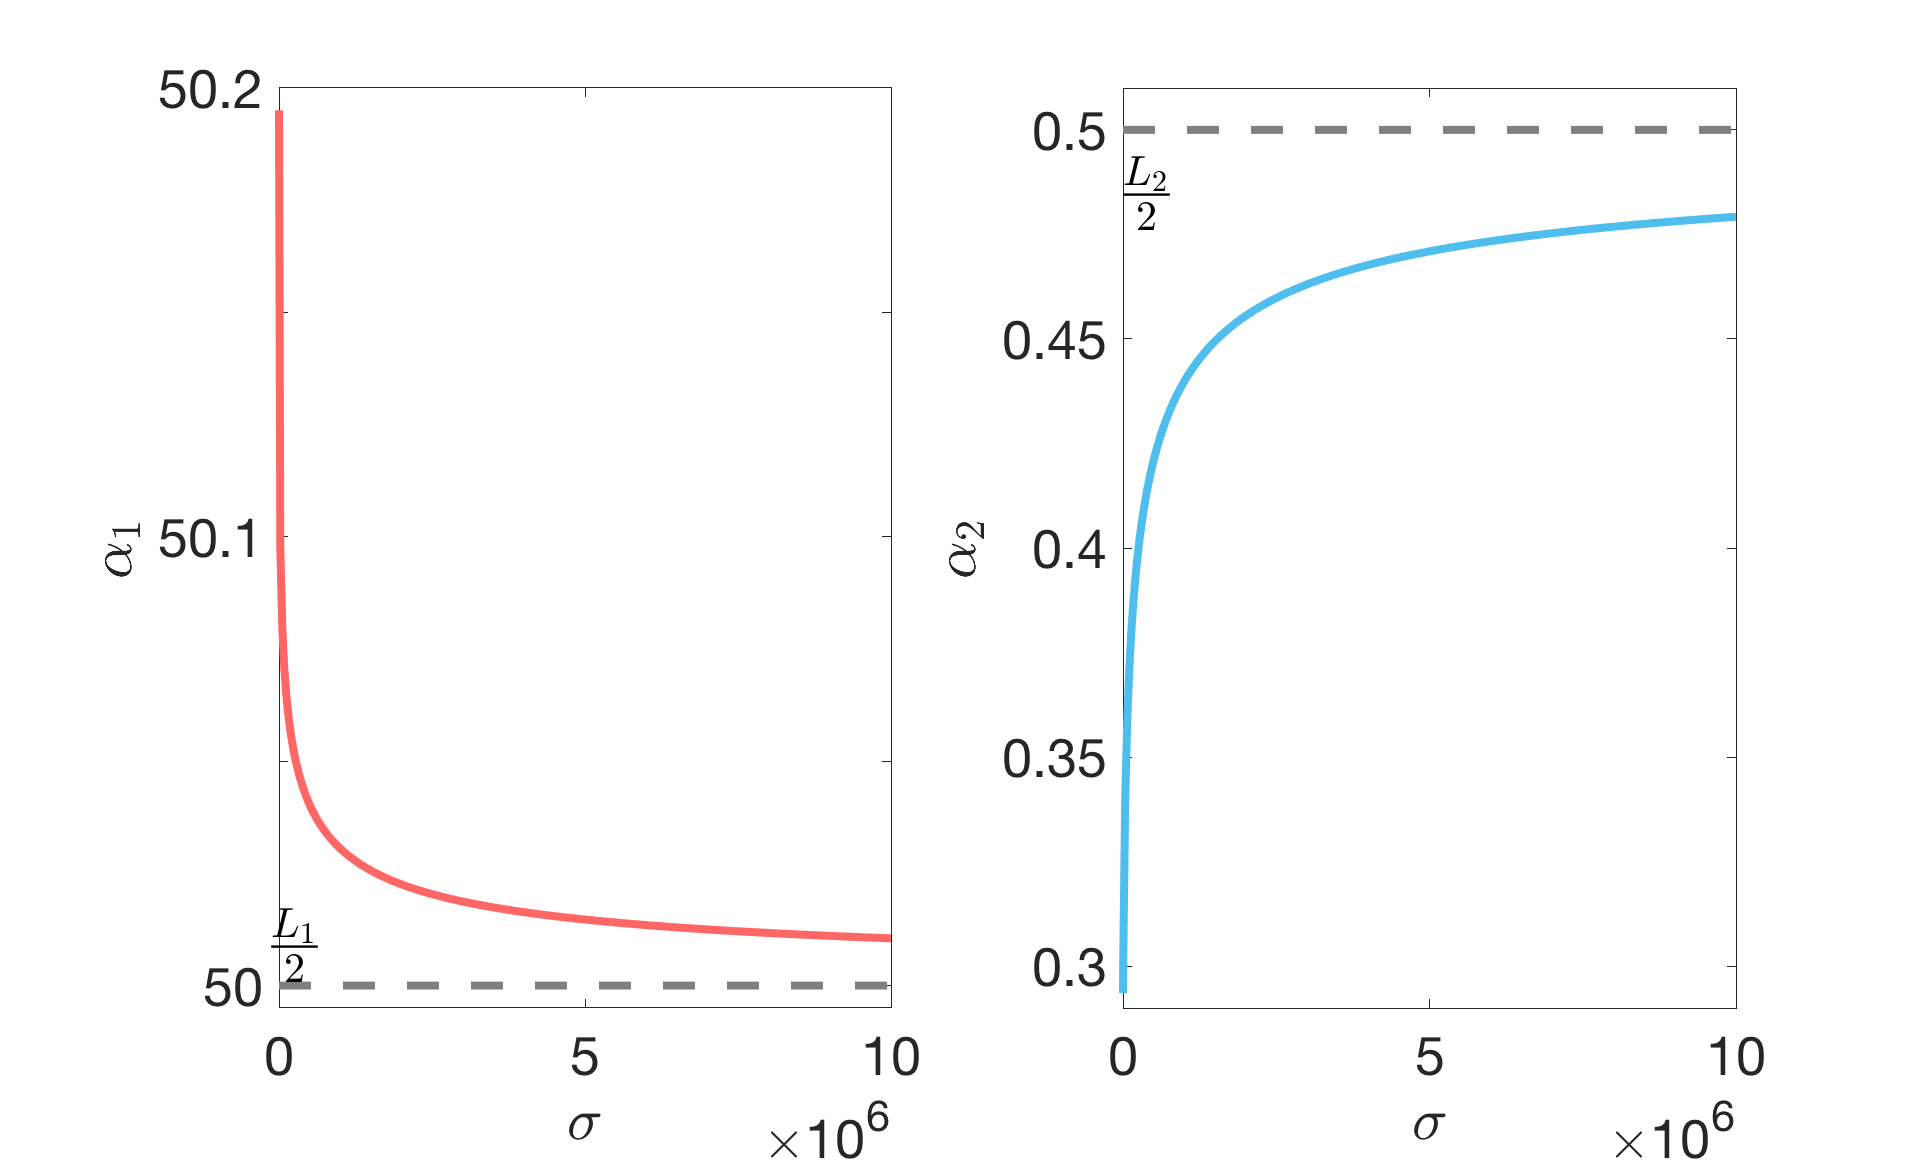
\includegraphics[width=0.9\textwidth]{figures/alpha.png}
    \caption{Plots of the function $\alpha_j(\sigma)$ for both slices in the hot phase $\left[\text{H}2,\text{H}2\right]$ solution. We chose a $\ell_2=10\ell_1$, $L_1=100\cdot L_2=100$ and a temperature where the hot phase dominates $\tau_2=2$. Both curves converge to $L_j/2$ as a result of the choice of the constant $c_j$.}
    \label{alpha_sigma}
\end{figure}

The solutions (\ref{solution x1}) and (\ref{solution x2}) give the limiting values of $x_j$. Since we are working in a symmetric geometry with respect to $\sigma = \sigma_+$, $x_j(\sigma)$ will take values in $]-\alpha_j(\sigma),\alpha_j(\sigma)[$ where $\alpha_j(\sigma)$ is given, up to a constant, by integrating eq. (\ref{solution x1}) and (\ref{solution x2}),
\begin{subequations}\label{mysolved}
\begin{align}
    \alpha_1(\sigma) = \frac{1}{2\pi T}\tanh^{-1}\left(\frac{\ell_1\left(\lambda^2+{\lambda_0}^2\right)}{2\lambda}\frac{1}{\sqrt{a_1\sigma+1}}\right) + c_1,\label{solved x1}\\
    \alpha_2(\sigma) = \frac{1}{2\pi T}\tanh^{-1}\left(\frac{\ell_2\left(\lambda^2-{\lambda_0}^2\right)}{2\lambda}\frac{1}{\sqrt{a_2\sigma+1}}\right) + c_2,\label{solved x2}
\end{align}
\end{subequations}
where $a_j=A\ell_j^2/4\lambda^2$. The constants are irrelevant in the computations. The choice $c_j=L_j/2$\footnote{not to be confused with the central charges.} fixes $x_j=0$ in the middle of the boundary interval $L_j$. The convention we are working in is that $\sigma$ increases as we circle the plane ($r_j,x_j$) clockwise.

We plotted these two function of $\sigma$ in fig. \ref{alpha_sigma}. We chose a temperature, $M_1=M_2=\left(2\pi T\right)^2$, where the hot phase already dominates over the warm phase.

\section{Conformal Compactification}

\begin{figure}
    \centering
    \begin{subfigure}[b]{0.45\textwidth}
        \centering
        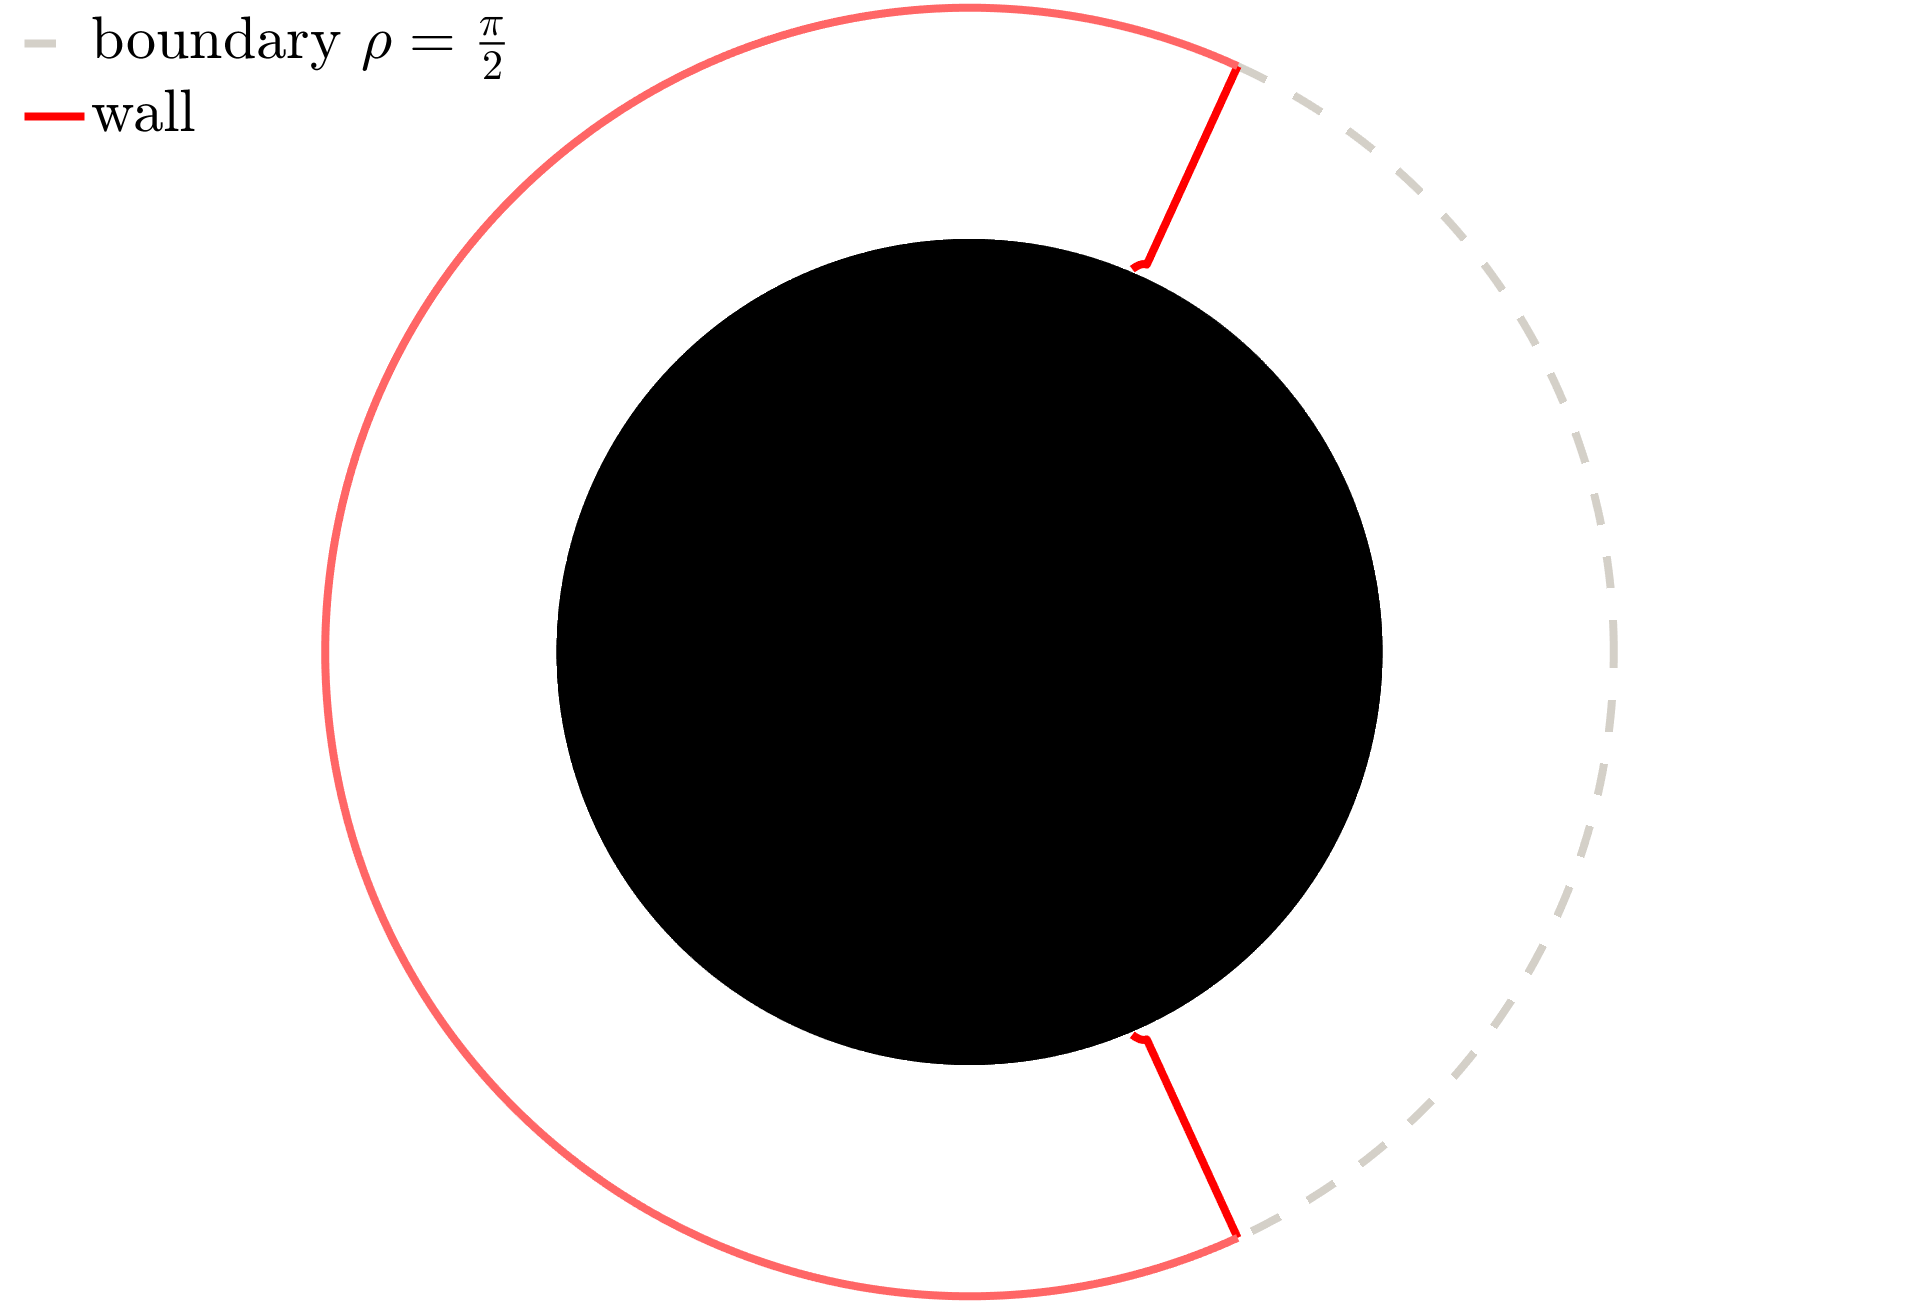
\includegraphics[width=\textwidth]{figures/wall_red.png}
        \label{wall_red}
    \end{subfigure}
    \hfill
    \begin{subfigure}[b]{0.45\textwidth}
        \centering
        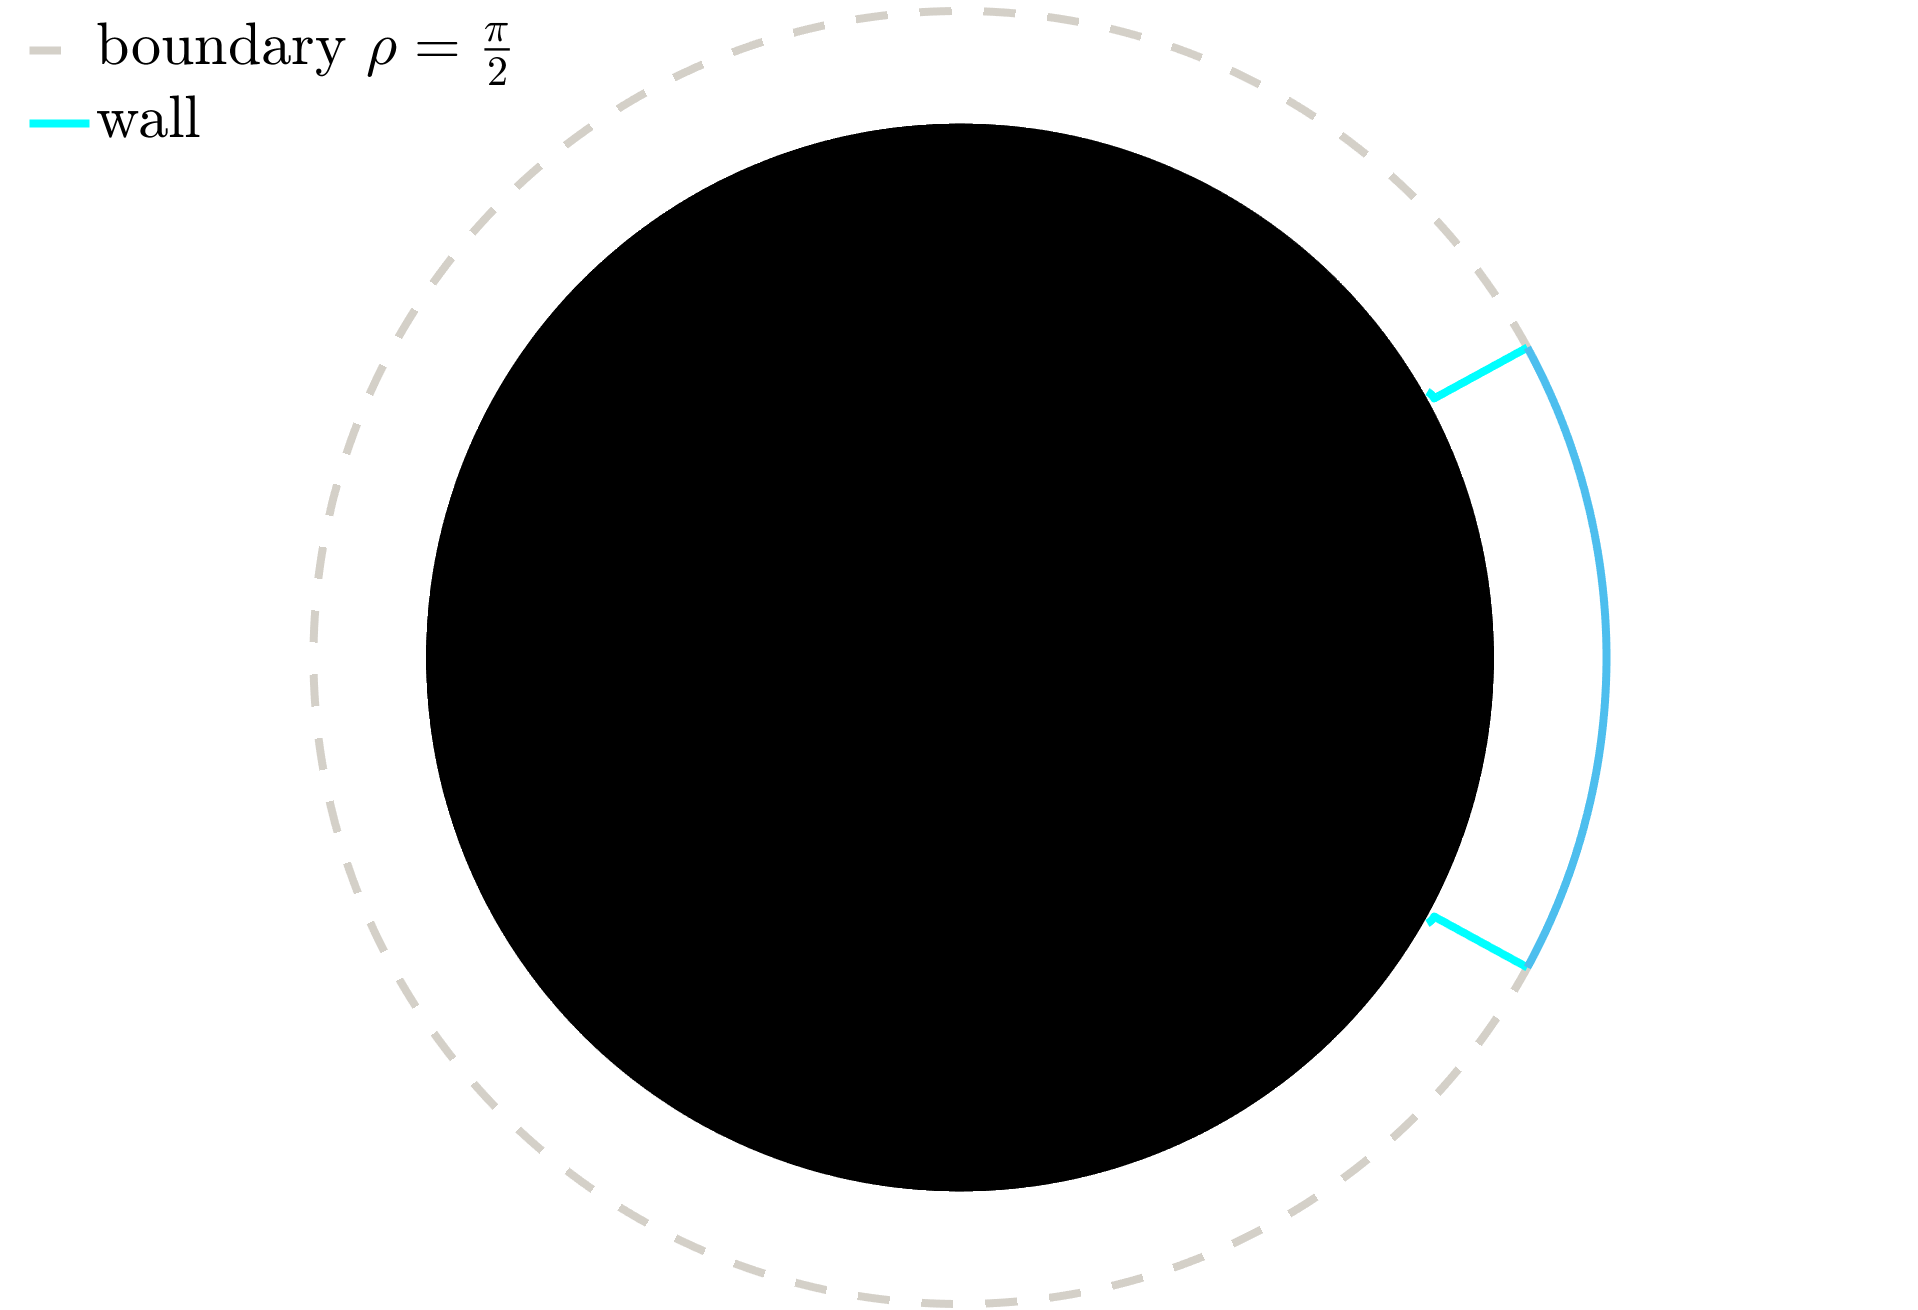
\includegraphics[width=\textwidth]{figures/wall_blue.png}
        \label{wall_blue}
    \end{subfigure}
    \caption{A plot of the wall (\ref{mysolved}) inside each slice.}
    \label{slicegeodesic}
\end{figure}


In order to get a good representation of the geometry we are working on, we make a change of variables to represent $r_j$ on a finite interval. We make the following change of coordinate,
\begin{equation}
    r=\tan{\rho}, \quad \text{where} \rho \in [0,\frac{\pi}{2}).
\end{equation}

The metric (\ref{geometry}) becomes,
\begin{equation}
    \text{d}s^2 = \frac{1}{\cos^2{\rho_j}}\left( \frac{\ell_j^2}{\sin^2{\rho_j}-M_j\ell_j^2\cos^2{\rho_j}}\text{d}\rho_j^2+\sin^2{\rho_j}\text{d}x_j^2\right)
\end{equation}
where we work at constant time, $\text{d}t=0$.

The horizon is found solving $g_{\rho\rho}^{-1}=0$, which gives $r_j = \tan\rho_j=\ell_j\sqrt{M_j}$. The conformal factor $\Omega^2(\rho_j)=\cos^{-2}(\rho_j)$ diverges at $\rho_j=\pi/2$.

The advantage of this compactification is that the representation now looks more like the spherical representations we had in previous figures. We use this change of coordinate to plot the wall solutions (\ref{mysolved}) inside the geometry. This is represented in fig. \ref{slicegeodesic}.
